\chapter{Estado da Arte}

Neste capítulo é apresentado o estado da arte relativo ao contexto desta dissertação. 

\section{Introdução ao problema}

A plataforma \gls{clav} pode ser divididas em 3 eixos principais:

\begin{enumerate}
    \item \textbf{Frontend}
    Responsável pela interação dos utilizadores com plataforma, bem como chamadas à \gls{api}, podendo esta ser de cariz público ou privado, através do acesso a certas funcionalidades da plataforma (por exemplo: listagens de utilizadores, entidades, legislações, etc).
    
    \item \textbf{Backend}
    Desenvolvido em \emph{NodeJS}, este é responsável por satisfazer os serviços requisitados pelo \emph{Frontend}. Inclui toda a lógica da aplicação, como a camada de acesso a dados, leitura e armazenamento de informação.
    
    \item \textbf{API de dados}
    Responsável pela comunicação e gestão de pedidos dos utilizadores da plataforma, sendo que a sua principal função é servir de elo de ligação entre os resultados guardados em base de dados e o \emph{Frontend} disponibilizado aos utilizadores.
\end{enumerate}

Devido à natureza dos dados presentes na plataforma \gls{clav}, foi necessário proceder a uma correta e estruturada implementação de diversos mecanismos de segurança e proteção contra uso indevido de dados.

\cleardoublepage
%\section{Soluções adoptadas}
%De modo a oferecer um nível de segurança adequado à plataforma, foram adotadas várias medidas de segurança, sendo estas explicadas em mais detalhe nas subsecções seguintes.

\section{Gestão de utilizadores}

A gestão de utilizadores é feita através da combinação entre o middleware\footnote{Middleware é um software que funciona como intermediário entre dois programas.} designado por \emph{Passport} e a base de dados não-relacional\footnote{Estilo de base de dados livres de esquema, capazes de maior escalabilidade que as base de dados tradiconais.} implementada em \emph{MongoDB}.

Devido à informação sensível que pode ser guardada na mesma, campos como a password são, naturalmente, encriptados recorrendo a técnicas discutidas posteriormente.

%\subsubsection{Passport}
O \emph{Passport} é um middleware de autenticação, desenvolvido para \emph{NodeJS}, com mais de 500 estratégias\footnote{Uma estratégia pode ser interpretado como um mecanismo único de autenticação.} diferentes de autenticação. Foi criado para solucionar um único problema: \textbf{autenticar pedidos}.

Devido à natureza do \emph{Passport}, este é extremamente fácil de implementar numa dada aplicação, devido ao seu forte encapsulamento e ao facto de delegar qualquer funcionalidade, que não seja a autenticação, para a aplicação.

Devido à natureza das aplicações Web modernas, a autenticação pode ser feita por diversas estratégias. A estratégia utilizada neste projeto recaiu sobre a escolha mais "tradicional", uma autenticação local com campos para \emph{username} e \emph{password}.

Embora com o aumento exponencial da popularidade de implementações de autenticação baseadas em redes sociais, através de protocolos baseados em \emph{OAuth}\footnote{Protocolo open-source que permite autenticação de forma standard e segura, entre aplicações desktop, web e mobile.}, tais como \emph{Google+} e \emph{Facebook}, foi decidido desde uma fase inicial que tais estratégias não seriam consideradas devido ao carácter profissional da plataforma.

Devido a cada aplicação possuir necessidades diferentes, o \emph{Passport} guarda cada estratégia de autenticação em módulos independentes, deixando assim a cargo do programador que estratégias empregar, sem criar dependências desnecessárias.

De seguida será apresentada a forma como as passwords dos utilizadores estão a ser protegidas.

\cleardoublepage
\subsection{Introdução à encriptação}

Em qualquer aplicação no mundo real, é impensável guardar dados sensíveis, como passwords, em formato \emph{plain-text}. Daí surgiu a necessidade de proteger informação sensível através de métodos designados por \emph{hashing}\footnote{Uma função hash é um algoritmo que mapeia dados de comprimento variável para dados de comprimento fixo.}.\\

\begin{figure}[h]
    \centering
    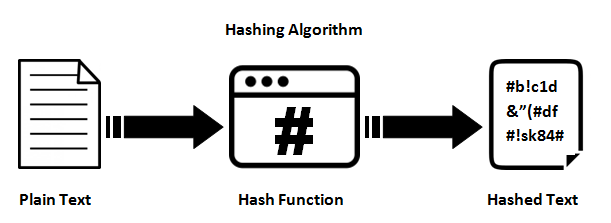
\includegraphics[width=0.75\textwidth]{img/bcrypt/Hashing.png}
    \caption{Representação de uma função de \emph{hash}.\cite{hashFunction}}
\end{figure}

Em geral, o \emph{hashing} é caraterizado como uma operação de sentido único, através da qual se gera um resultado único, impossível de reverter para o texto original.
Embora esta noção esteja correta e seja de facto impossível, através de um texto já processado por uma função de \emph{hash}, reconstruir o texto original em questão, este não é infalível.

\cleardoublepage
\subsubsection{Vulnerabilidades}

Para exemplificar vulnerabilidades existentes nas funções criptográficas que recorrem apenas ao \emph{hashing} de passwords, vamos recorrer ao algoritmo \textbf{SHA-1}, pertencente à familia de algoritmos \gls{sha}.

O principal problema das funções da família \gls{sha} assenta no facto de que foram desenvolvidas para serem computacionalmente rápidas. A rapidez com que uma função pode calcular \emph{hashes}, tem um impacto imediato e significativo na quão seguro uma password é.

Embora cálculos mais rápidos levem ao desenvolvimento de algoritmos mais eficientes a nível de computação, também abrem portas a ataques \emph{bruteforce}. Atualmente, com o auxilio de \gls{cpu} e \gls{gpu} modernas, é possível calcular milhões, ou até bilhões de \emph{hashes} por segundo.

Outro problema assenta no facto que qualquer função responsável por \emph{hashing}, para o mesmo texto, retorna sempre o mesmo resultado de \emph{hash}, como podemos verificar na tabela seguinte.

\begin{center}
    \begin{tabular}{ |p{2cm}|p{2cm}|p{8cm}|  }
        \hline
        \multicolumn{3}{|c|}{Resultados do algoritmo SHA-1} \\
        \hline
        Utilizador & Password & \emph{Hashed} password\\
        \hline
        \textcolor{red}{António} & \textcolor{red}{12345} & \textcolor{red}{\textbf{8cb2237d0679ca88db6464eac60da96345513964}}\\
        Alice & sup3rs3gur4 & 0ce594a80be23686fa95527e219ff162291f80f0\\
        Manuel & uncrackabl3 & c4f9036ecefde84b5a8dc4296abbab1a6c53be60\\
        \textcolor{red}{Gustavo} & \textcolor{red}{12345} & \textcolor{red}{\textbf{8cb2237d0679ca88db6464eac60da96345513964}}\\
        Joana & 1a2b3c4d & b01afc2b077956acc69f99e0b7df1cb70cb01331\\
        \hline
    \end{tabular}
\captionof{table}{Aplicação do algoritmo \emph{SHA-1} a um conjunto de passwords.}\label{tab:sha1} 
\end{center}

Como exemplificado na Tabela \ref{tab:sha1}, o utilizador \textbf{António} e \textbf{Gustavo} partilham a mesma password, logo o resultado após o \emph{hashing} da mesma é idêntico. 

Embora passwords idênticas sejam extremamente comuns, o facto do \emph{hash} resultante ser idêntico apresenta um fator de risco muito mais elevado do que as passwords serem idênticas, pois estaria a expor um número exorbitante de utilizadores a uma grave falha de segurança.

Porém, o simples acto de \emph{hashing} de passwords não é uma solução segura. Este rapidamente foi descartado devido a ser extremamente suscetível a ataques baseado em \emph{rainbow tables}, também conhecidos por \emph{ataques de dicionário}.

Este ataque tem como base o facto de algoritmos como o \emph{SHA-1} ser extremamente rápido e eficiente, sendo que em vez de calcular em tempo real \emph{hashes} aleatórios, utilizam valores de hash pré-calculados para toda e qualquer possível combinação de caracteres, utilizando para validação o método \emph{bruteforce}.

Esta vulnerabilidade foi de tão larga escala, que poderia quebrar \emph{99.9\%} de todas as combinações possíveis de 14 caracteres alfanuméricos em 11 minutos (utilizando a \emph{rainbow table} menos extensa, sendo que com tabelas mais extensas esta figura descia consideravelmente).


%\cleardoublepage
\subsubsection{Melhorias no processo de hashing}

De modo a solucionar o problema anterior, é necessário implementar uma função de \emph{hashing} mais lenta, que seja eficaz na proteção de informação e capaz de abrandar, ou evitar possíveis ataques. Também é necessário que esta função seja adaptativa, ou seja, que devido a avanços tecnológicos em hardware esta se possa adaptar para ter um desempenho similar aos níveis atuais.

De modo a solucionar o problema proveniente de ataques \emph{bruteforce} baseados no uso de \emph{rainbow tables}, foi necessário diversificar ainda mais os \emph{hashes} gerados. Para tal foi adicionado um \emph{salt}\cite{sriramya2015providing}, de modo a fazer qualquer password verdadeiramente única.

De acordo com a \gls{owasp}, o \emph{salt} é um valor aleatório de tamanho fixo, considerado criptograficamente forte, que é adicionado ao input de uma dada função de \emph{hash}, independentemente deste do input ser ou não único.

Na tabela seguinte podemos verificar a importância de utilizar a técnica de \emph{salting} juntamente com o \emph{hashing} de passwords.

\begin{center}
    \begin{tabular}{ |p{1.7cm}|p{2cm}|p{1.5cm}|p{8cm}|  }
        \hline
        \multicolumn{4}{|c|}{Resultados do algoritmo SHA-1 c/ salting} \\
        \hline
        Utilizador & Password & Salt &\emph{Hashed} password + \textbf{salt}\\
        \hline 
        \textcolor{red}{António} & \textcolor{red}{12345} & r8ZGQH & c783b62c876b77310818b3b4cc6863ca008f7d10\\
        Alice & sup3rs3gur4 & yvL9H8 & d68c7166f916b91b66dda685e8eee1af70528933\\
        Manuel & uncrackabl3 & C4uHRv & 87d8e4e7ae79ab2487133a6513e35cb511687d5a\\
        \textcolor{red}{Gustavo} & \textcolor{red}{12345} & jKM2Lh & f69e3288fc17c383cab12aa78a725d675610e81a\\
        Joana & 1a2b3c4d & WNj7Vt & 866038b3d43de9a9b0b49a6ee1ffc6cbf64d3c6d\\
        \hline
    \end{tabular}
\captionof{table}{Aplicação do algoritmo \emph{SHA-1} com auxílio de \emph{salting} a um conjunto de passwords.}\label{tab:sha1_salt} 
\end{center}

Como exemplificado na Tabela \ref{tab:sha1_salt}, embora o utilizador \textbf{António} e \textbf{Gustavo} partilhem a mesma password, o resultado do \emph{hashing} é diferente.

Facilmente chegamos à conclusão que o \emph{salting} é essencial para manter a segurança de informação importante como passwords, pois um conjunto infinito de passwords idênticas nunca terão o mesmo \emph{hash}.

Embora seja teoricamente possível quebrar este tipo de combinação, esta requer poder computacional exponencialmente maior que um simples ataque \emph{rainbow table}, visto que o \emph{salt} é totalmente aleatório, tornando qualquer ataque inviável.

Em suma, o método de autenticação ideal deve implementar ambos estes métodos\cite{contini2015method}, \emph{hashing} e \emph{salting}, sendo que um dos métodos mais comuns e seguros da atualidade, é o \emph{bcrypt}, tornando-a no perfeito candidato para utilização neste projeto.

\cleardoublepage
\subsection{bcrypt}

De modo a solucionar os problemas referidos na secção anterior, foi necessário proceder ao desenvolvimento de uma função criptográfica que não só solucionasse o problema relacionado com ataques via \emph{rainbow tables}, mas também fosse capaz de acompanhar os avanços tecnológicos a nível computacional.

Para tal, Niels Provos e David Mazières desenvolveram a função de \emph{hashing} designada por \textbf{bcrypt}\cite{provos1999future}. Esta foi apresentada em 1999 na \gls{usenix}, sendo uma função baseada na cifra \emph{Blowfish}, desenvolvia por Bruce Schneier e apresentada em 1993.

Além de incorporar um \emph{salt} para proteger contra ataques via \emph{rainbow tables}, esta foi desenvolvida para ser uma função adaptável, sendo que o número de iterações pode ser incrementado de modo a aumentar o número de ciclos máquina necessários para o cálculo do \emph{hash}. 

\begin{algorithm}
    \caption{Pseudo código do algoritmo \emph{bcrypt}.}
    \begin{algorithmic}[1]
        \Function{bcrypt}{cost, salt, pwd}
        \State $state\gets EksBlowfishSetup(cost,salt,key)$
        \State $ctext\gets OrpheanBeholderScryDoubt$
        \State \textbf{repeat}(64)
        \State \indent $ctext\gets EncryptECB(state, ctex)$
        \State \textbf{return} Concatenate(cost, salt, ctext)
    \EndFunction
    \end{algorithmic}
\end{algorithm}

Através do pseudo código acima descrito, é possível verificar que o algoritmo \emph{bcrypt} devolve uma string composta pelo custo, \emph{salt} e o hash da password.

Utilizando como exemplo a string "octavio" com um fator de custo 12, o algoritmo \emph{bcrypt} retorna o seguinte:

\begin{center}
    \textbf{\textcolor{red}{\$2y\$}\textcolor{green}{12\$}\textcolor{blue}{au1FX9q7Ju67N3INnoBo3uYqKrkYRLPFH1}\textcolor{orange}{.ycZ4GU9qHuo6c2FaN6}}
\end{center} 

Esta string pode ser dividida em 4 secções:

\begin{itemize}
    \item Versão do \emph{bcrypt} utilizada (representada a vermelho).
    \item Fator de custo, valor entre 1 e 31 (representada a verde).
    \item String correspondente ao \emph{salt} (representada a azul).
    \item Password após \emph{hash} da mesma(representada a laranja).
\end{itemize}

A combinação destas duas técnicas faz com que, até à data de publicação desta pré-dissertação, o algoritmo \emph{bcrypt} ainda não tenha sido quebrado, sendo que se trata do algoritmo escolhido por sistemas operativos como o \emph{OpenBSD} e \emph{SUSE Linux} para o \emph{hashing} das suas passwords.

Esta fama levou a que o \emph{bcrypt} seja considerado por muitos, o standard da indústria em termos de encriptação de passwords.

\subsubsection{Funcionamento do bcrypt}

De modo a proporcionar uma forma de aumentar o tempo computacional o algoritmo \emph{bcrypt}, Niels Provos e David Mazières basearam-se na cifra \emph{Blowfish} já existente, criando assim uma versão designada por \emph{Eksblowfish} (\textit{\textbf{Expensive key schedule} Blowfish}).

\begin{algorithm}
    \caption{Pseudo código do algoritmo \emph{EksBlowfish}.}
    \begin{algorithmic}[1]
        \Function{EksBlowfishSetup}{cost, salt, key}
        \State $state\gets InitState()$
        \State $state\gets ExpandKey(state, salt, key)$
        \State \textbf{repeat}($2^{cost}$)
        \State \indent $state\gets ExpandKey(state, 0, salt)$
        \State \indent $state\gets ExpandKey(state, 0, key)$
        \State \textbf{return} state
    \EndFunction
    \end{algorithmic}
\end{algorithm}

Esta alteração à cifra \emph{Blowfish} não foi feita com o intuito de a tornar criptograficamente mais forte, mas sim alterar a forma como a \emph{key} é calculada.

Tendo em consideração que a \emph{key} é um valor aleatório variável entre 1 e 72 bytes, inclusive, esta alteração torna o cálculo da \emph{key} demoroso a nível computacional (\textbf{Expensive}).

De modo a prolongar o tempo de execução desta função, é aplicada a expansão da \emph{key} $2^{cost}$ vezes. Esta alteração é a maior distinção entre o algoritmo \emph{Blowfish} original e o \emph{Eksblowfish}, sendo a causa do \emph{bcrypt} ser considerado um algoritmo adaptável.

No gráfico seguinte, podemos ver uma relação entre o factor de custo e o tempo de execução do algoritmo \emph{bcrypt}. \textbf{(teste efetuado com processador Intel Core i7-4770K 4c/8t)}

\begin{center}
    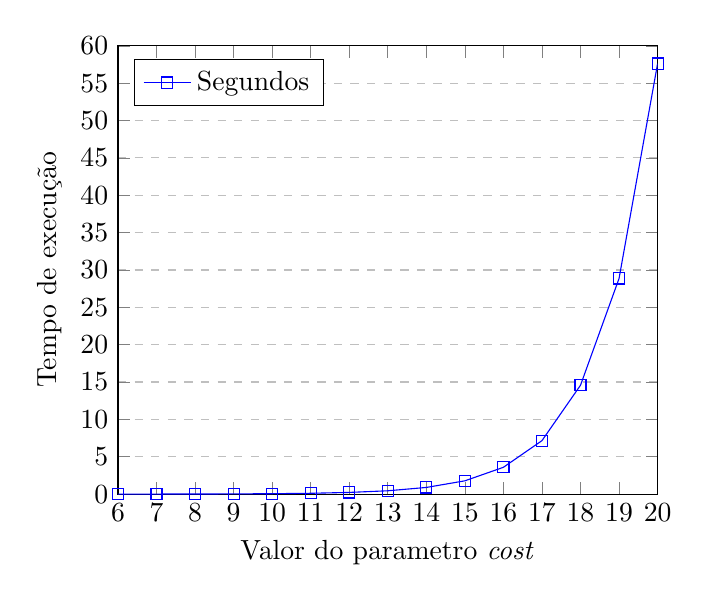
\begin{tikzpicture}
        \begin{axis}[
            xlabel={Valor do parametro \emph{cost}},
            ylabel={Tempo de execução},
            xmin=6, xmax=20,
            ymin=0, ymax=60,
            xtick={6,7,8,9,10,11,12,13,14,15,16,17,18,19,20},
            ytick={0,5,10,15,20,25,30,35,40,45,50,55,60},
            legend pos=north west,
            ymajorgrids=true,
            grid style=dashed,
        ]
        \addplot[
            color=blue,
            mark=square,
            ]
            coordinates {
            (6,0.003622)(7,0.007590)(8,0.013918)(9,0.028723)(10,0.055023)(11,0.110837)(12,0.226982)(13,0.446507)(14,0.892617)(15,1.778647)(16,3.588397)(17,7.155973)(18,14.572114)(19,28.860461)(20,57.623139)
            };
            \legend{Segundos}
        \end{axis}
    \end{tikzpicture}
\end{center}

\cleardoublepage
\subsubsection{bcrypt no mundo real}

Como foi mencionado nas secções prévias, um dos factos de o \emph{bcrypt} ainda ser utilizado deve-se não só à sua segurança, mas ao facto de acompanhar as evoluções tecnológicas a nível de processamento.

Quando foi originalmente lançado em 1999, devido ao tempo de execução do algoritmo \emph{bcrypt} ser adaptável, começou por ser utilizado um fator de custo de 6, pois este era o valor para o qual resultava um tempo de execução de aproximadamente 250ms (considerado por muitos o \emph{standard}).

Devido a enormes avanços tecnológicos, hoje em dia um fator de custo 6 na máquina previamente descrita leva a um tempo de execução de apenas 3.6ms, ou seja, aproximadamente 70 vezes menor do que em 1999.

Para combater esta crescente incessável de poder computacional, o fator de custo deve ser ajustado de acordo com o hardware atual, sendo que hoje em dia o fator de custo mais comum é de 12 a 14, o que nosso teste levou a um tempo de execução entre 226ms e 890ms.

De modo a exemplificar a importância do fator de custo, vamos imaginar o seguinte cenário:

\begin{itemize}
    \item Aplicação com 1000 utilizadores, cujas passwords estão contida num dos conjuntos em baixo especificados.
    \item Conjunto de passwords mais usadas:
    \begin{enumerate}
        \item 100 passwords.
        \item 1000 passwords.
        \item 10000 passwords.
    \end{enumerate}
    \item É permitido tentativas de autenticação ilimitadas, eliminando assim qualquer defesa contra ataques \emph{bruteforce}.
\end{itemize}

Quanto tempo demoraria a um atacante, com um processador idêntico ao descrito anteriormente, testar todas as passwords para os 1000 utilizadores?

\begin{center}
    \begin{tabular}{ |p{2.5cm}|p{3cm}|p{3cm}|p{3cm}|  }
        \hline
        \multicolumn{4}{|c|}{Tempo necessário para testar todas as passwords para os 1000 utilizadores.} \\
        \hline
        Fator de custo & 100 passwords & 1000 passwords & 10000 passwords\\
        \hline 
        6 & 6 minutos & 1 hora & 10 horas\\
        7 & 12 minutos & 2 horas & 21 horas\\
        8 & 23 minutos & 4 horas & 2 dias\\
        9 & 48 minutos & 8 horas & 3 dias\\
        10 & 92 minutos & 15 horas & 6 dias\\
        11 & 3 horas & 30 horas & 13 dias\\
        12 & 6 horas & 3 dias & 1 mês\\
        13 & 12 horas & 5 dias & 2 meses\\
        14 & 1 dia & 10 dias & 3 meses\\
        15 & 2 dias & 21 dias & 7 meses\\
        16 & 4 dias & 1 mês & 1 ano\\
        17 & 1 semana & 3 meses & 2 anos\\
        18 & 2 semanas & 6 meses & 5 anos\\
        19 & 1 mês & 11 meses & 9 anos\\
        20 & 2 meses & 2 anos & 18 anos\\
        \hline
    \end{tabular}
\captionof{table}{Tempo necessário para testar combinações de passwords para 1000 utilizadores.}\label{tab:bcrypt_bruteforce} 
\end{center}

Facilmente percebemos que fatores de custo como 10 são demasiado baixos para a atualidade, sendo imperativo a escolha de um fator de custo equilibrado. Outro facto a ter em consideração é este teste ter sido feito com um processador \emph{mainstream}, sendo que o mesmo se encontra 4 gerações atrasado em comparação com a atual 9ª geração de processadores Intel.

Outro problema que tem ganho tração nos últimos anos, é o aparecimento de soluções especializadas sobre a forma de \gls{gpu}, \gls{fpga}\cite{wiemer2014high}\cite{malvoni2014your} e \gls{asic}, capazes de poder computacional extremamente superior, quando comparados com o \gls{cpu} utilizado para os testes anteriores.

Um \gls{fpga} é um circuito integrado que tem a possibilidade de ser reprogramado através de \emph{bitstreams}, de modo a ser utilizado em aplicações diferentes, como por exemplo, cálculos de hash baseados no algoritmo SHA-1, SHA-256, etc. Enquanto que um \gls{asic}, embora também seja um circuito integrado, apenas consegue fazer uma função e não pode ser reprogramado, no entanto oferece performance muito superior a um \gls{fpga}.

Na tabela seguinte exploramos a performance em hashes por segundo (H/s) entre \gls{cpu}\footnote{\gls{cpu} fabricado pela Intel, desenvolvido na arquitetura \emph{Sandy Bridge}.}, \gls{gpu}\footnote{\gls{gpu} fabricada pela NVIDIA, desenvolvida na arquitetura \emph{Maxwell}.} e \gls{fpga}\footnote{Ambos os \gls{fpga} utilizados para comparação são desenvolvidos pela Xilinx.} relativamente ao algoritmo \emph{bcrypt}.

\begin{center}
    \begin{tabular}{ |p{1cm}|p{2.5cm}|p{2cm}|p{2cm}|p{1.75cm}|p{0.9cm}|  }
        \hline
        \multicolumn{6}{|c|}{Cálculo de hashes por segundo (H/s) em diverso hardware.} \\
        \hline
        Tipo & Modelo & Custo 6 & Custo 12 & Consumo & Preço\\
        \hline
        CPU & Xeon E3-1240 & 6210 H/s & 50 H/s& 300W & 262\$\\
        GPU & GTX 750Ti & 1920 H/s& 15 H/s& 300W & 120\$\\
        FPGA & zedboard & 6511 H/s & 51.95 H/s& 4.2W & 319\$\\
        FPGA & Virtex-7 & 51437 H/s& 410.4 H/s& 20W & 3495\$\\
        \hline
    \end{tabular}
\captionof{table}{Comparação entre hardware no cálculo de H/s, eficiência e custo.\cite{wiemer2014high}}\label{tab:bcrypt_hashrate} 
\end{center}

Mais uma vez é possível identificar outro um problema que não foi previamente considerado: como ajustar o fator de custo para este tipo de hardware especializado, como por exemplo \gls{fpga} e \gls{asic}?

Infelizmente a resposta é que este ajuste é deveras impossível. O simples aumento do fator de custo é impensável, pois iria implicar tempos exponenciais de computação em \gls{cpu} mainstream.

Felizmente, tal aplicação de hardware pare este efeito ainda não foi detetada no mundo real e não aparenta qualquer problema de momento.

\cleardoublepage
\subsection{Armazenamento e validação de sessões}

De modo a fazer uma gestão de utilizadores mais aprofundada, foi necessário implementar métodos capazes de não só limitar o número de utilizadores ativos a cada dado momento, mas também manter as sessões iniciadas no caso de falha do servidor.

Numa primeira fase do projeto \gls{clav} foi implementada uma solução baseada em \emph{JSON Web Token}, que será explicada na subsecção seguinte. Embora esta se tenha provado eficaz, a mesma não era capaz de manter as sessões iniciadas no caso de uma falha súbita do servidor, ou seja, se o servidor por algum motivo sofresse de uma falha de energia e tivesse de reiniciar, devido às sessões estarem guardadas localmente, as mesmas eram perdidas.

Outro fator decisivo contra esta implementação assenta no facto de não ser possível recorrer ao paralelismo da aplicação através do \emph{nginx}\footnote{Mais informação em \url{https://www.nginx.com}}, pois a comunicação entre processos paralelos não permite a partilha do token guardado localmente.

Para tal, foi necessário recorrer a outra abordagem, o armazenamento de sessões em base de dados, neste caso em \emph{MongoDB}.

\subsubsection{Validação através de JSON Web Token}

Durante o desenvolvimento do projeto \gls{clav} foi discutida a implementação de um mecanismo capaz de terminar sessões automaticamente, de modo a diminuir o número de sessões ativas, bem como evitar possíveis falhas de segurança.

Para tal foi implementado, juntamente com o \emph{Passport}, uma estratégia capaz de lidar com \gls{jwt}, representada através do seguinte pseudo código.

\begin{algorithm}
    \caption{Pseudo código da autenticação via \emph{JSON Web Token}.}
    \begin{algorithmic}[1]
        \Function{JwtStrategy}{opts, jwt\_payload, done}
        \State $user \gets findUserByJwt(jwt\_payload.id)$
        \If {$user \neq invalid$}
            \State \textbf{return} done(null, user)
        \Else
            \State \textbf{return} done(null, false)
        \EndIf
    \EndFunction
    \end{algorithmic}
\end{algorithm}

Como explicado na secção anterior, através do uso do \emph{JSON Web Token} é possível passar no atributo \emph{exp} uma data de expiração, após a qual o token se torna inválido, terminando assim a sessão do utilizador.

Para tal, quando a estratégia de login local do \emph{Passport} é invocada, é necessário proceder à assinatura de um token \gls{jwt} e atribuí-lo à sessão do utilizador atual.

\begin{algorithm}
    \caption{Pseudo código da atribuição de um \gls{jwt} à sessão.}
    \begin{algorithmic}[1]
        \Function{login}{user}
        \State $token \gets jwt.sign({user}, jwt.secret, \{$
        \State \indent $expiresIn : jwt.expiration$
        \State $\}$
        \State $session.token \gets token$
    \EndFunction
    \end{algorithmic}
\end{algorithm}

Os valores de \emph{secret} e \emph{expiration} previamente utilizados são provenientes de um ficheiro externo, no qual designamos a duração (em segundos) em que a sessão está ativa, bem como a chave secreta utilizada para a assinatura.

\begin{verbatim}
    jwt: {
        secret: 'ihfH6Cv4LVD1YoG...vY8XdVch5ebGHTdPMDGHy',
        expiration: 3000 //in seconds
    }
\end{verbatim}

Após corretamente atribuída a sessão a um utilizador, cada vez que o mesmo pretende aceder a páginas restritas, como por exemplo, a adição de entidades à plataforma \gls{clav} é realizada uma chamada ao \emph{middleware} de autenticação \emph{isLoggedIn}, o qual verifica se existe um utilizador com sessão iniciada, bem como se o token do mesmo ainda não expirou, sendo esta lógica representada através do seguinte pseudo código.

\begin{algorithm}
    \caption{Pseudo código da função  de middleware \emph{isLoggedIn}.}
    \begin{algorithmic}[1]
        \Function{isLoggedIn}{req, res, next}
        \If {$req.isAuthenticated()$}
        \State $result \gets jwt.verify(session.token, jwt.secret)$
            \If {$result \neq expired$}
                \State \textbf{return} next()
            \Else
                \State \textbf{return} err
            \EndIf
        \EndIf
    \EndFunction
    \end{algorithmic}
\end{algorithm}

Embora esta implementação do \emph{JSON Web Token} estivesse 100\% funcional, a mesma foi abandonada da gestão de utilizadores por uma alternativa similar, o armazenamento de sessões ativas diretamente na base de dados em \emph{MongoDB}, sendo apenas utilizado o \gls{jwt} na autenticação de pedidos à \gls{api}.

\cleardoublepage
\subsubsection{Armazenamento em MongoDB}

O armazenamento de sessões em \emph{MongoDB} permite uma maior flexibilidade comparativamente com o armazenamento local.

Em primeiro lugar é possível recorrer ao paralelismo da aplicação via \emph{nginx} ou outras soluções similares, pois cada \emph{thread} pode correr independentemente umas da outras e a comunicação entre processos paralelos passa a ser inexistente. Para validar sessões cada \emph{thread} faz uma \emph{query} à base de dados, verificando se a sessão do utilizador é válida.

Permite também que na ocorrência de uma falha súbita do sistema, as informações relativas às sessões não se percam devido a estarem armazenadas em base de dados. Assim sendo, após o \emph{boot} do sistema, os utilizadores continuam com as sessões ativas, algo que não aconteceria se fosse utilizado armazenamento local e validação via \gls{jwt}.

Um possível problema desta solução seria que iríamos delegar o armazenamento das sessões para o lado do servidor, ou seja, se por ventura existissem milhões de sessões armazenadas, iria ser ocupado um tamanho substancial de memória em disco. Para evitar tal problema, é utilizado o módulo \emph{\textbf{connect-mongo}}\footnote{\url{https://github.com/jdesboeufs/connect-mongo}} que permite a auto remoção de sessões expiradas, bem como a atribuição de um tempo máximo após o qual a sessão expira.

Para atingir este objetivo, apenas é necessário adicionar os campos abaixo mencionados à sessão do \emph{ExpressJS}.

\begin{verbatim}
    app.use(session({
        ...
        autoRemove: 'interval',
        autoRemoveInterval: 15, //minutes
        store: new MongoStore({
            url: dataBases.userDB,
            ttl: 1800 //seconds
        })
    }));
\end{verbatim}

Esta configuração do módulo \emph{\textbf{connect-mongo}} faz com que a cada 15 minutos seja invocada a função de remoção de sessões expiradas, sendo que cada sessão apenas é válida durante 1800 segundos, ou seja, 30 minutos.

Em suma, o armazenamento de sessões em base de dados possui todas as qualidades da validação via \emph{JSON Web Token}, oferecendo uma maior flexibilidade e customização, sem impacto na performance do servidor.

\cleardoublepage
\section{Autenticação através do Auth.Gov}

O Autenticação.Gov surge da necessidade de identificação unívoca de um utilizador perante sítios na Web. Cabe a esta solução o processo de autenticação e o fornecimento dos atributos do utilizador necessários a que cada entidade possa efetuar a identificação do utilizador.

O Autenticação.Gov, em conjunto com o \gls{cc}, também permite fazer uso da funcionalidade de Federação de Identidades da Plataforma de Interoperabilidade da Administração Pública para a identificação sectorial de um Cidadão, isto é, a obtenção dos seus identificadores junto das entidades participantes da iniciativa do Cartão de Cidadão. É também responsável pela gestão dos vários fornecedores de atributos disponíveis e possui uma estreita ligação com a infraestrutura de chave pública do Cartão de Cidadão (\gls{pki}), com o intuito de manter elevados níveis de segurança e privacidade no processo de autenticação e identificação.

Através do Autenticação.Gov é possível a criação de credenciais comuns a todos os sites da Administração Pública, assegurando que o utilizador se necessita de autenticar apenas uma única vez para executar um ou vários serviços que podem ser iniciados em portais transversais (como o Portal do Cidadão ou o Portal da Empresa).

Permite também proceder à autenticação de um utilizador com recursos a outros certificados digitais que não o do Cartão de Cidadão, possibilitando e alargando o leque de autenticação disponível para as Entidades que pretendam delegar a autenticação nesta componente.

Em seguida podemos verificar a quantidade de utilizadores únicos e autenticações realizadas com o auxílio da plataforma \emph{Autenticação.Gov}.

\begin{figure}[h]
    \centering
    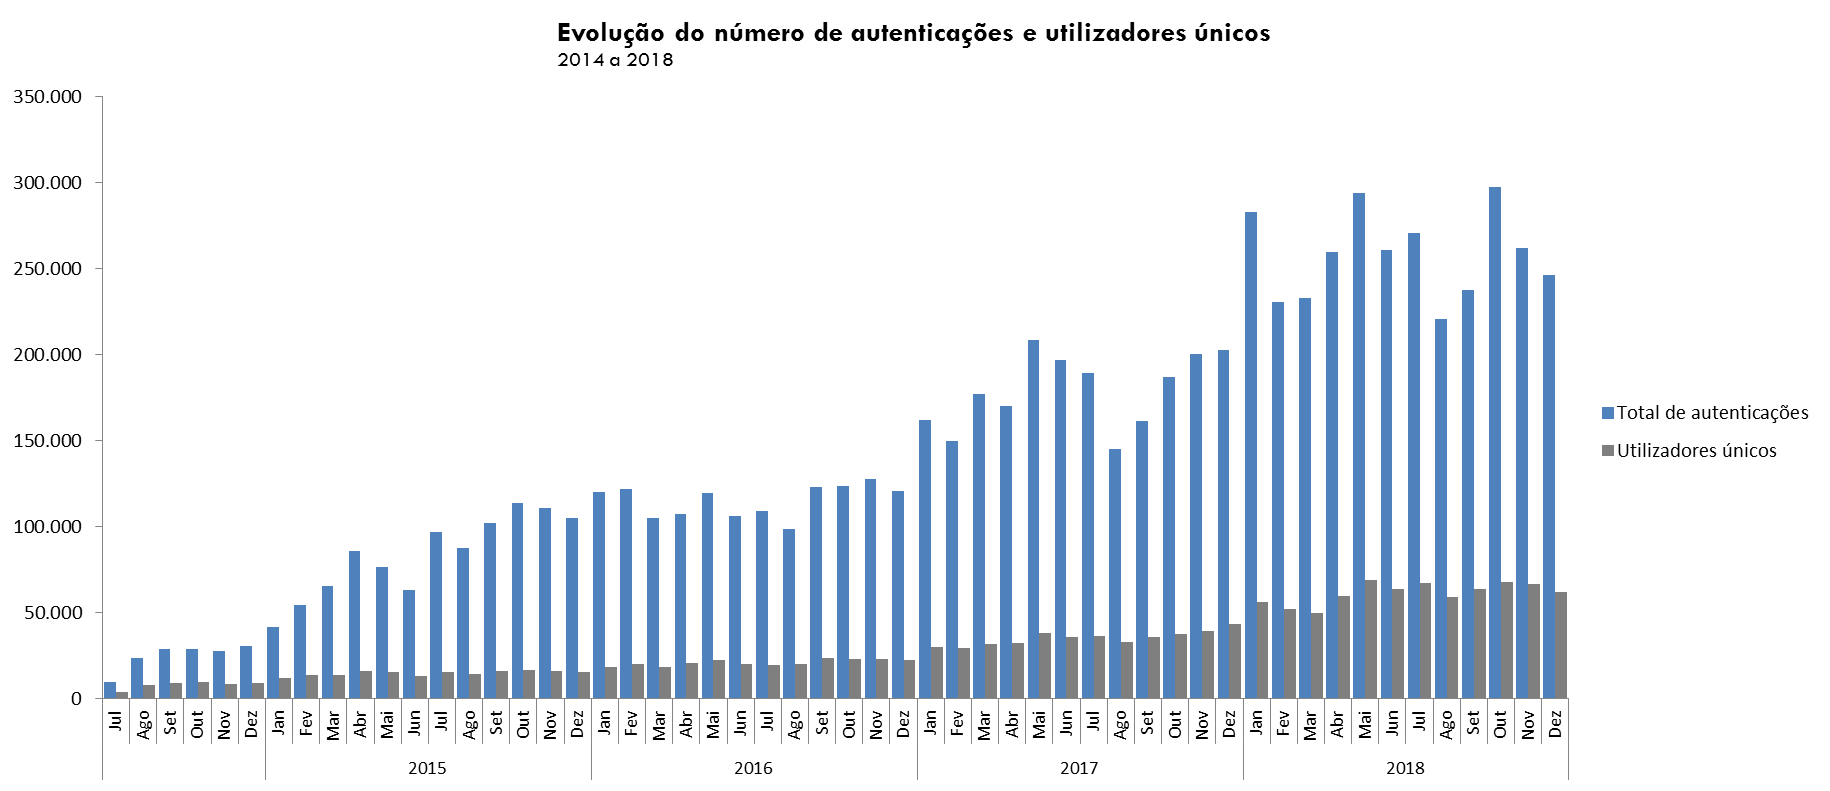
\includegraphics[width=\textwidth]{img/authgov/authgovusage.png}
    \caption{Evolução do número de autenticações realizadas e utilizadores únicos baseados na plataforma \emph{Autenticação.Gov}.\cite{authGovStats}}
\end{figure}

\begin{figure}[h]
    \centering
    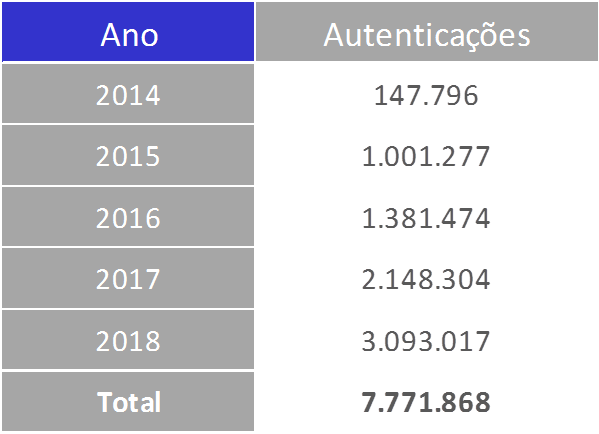
\includegraphics[width=0.5\textwidth]{img/authgov/authAnos.png}
    \caption{Representação do número total de autenticações realizados com a plataforma \emph{Autenticação.Gov}.\cite{authGovStats}}
\end{figure}

Relativamente ao âmbito do projeto \gls{clav} irá ser implementada a autenticação através dos seguintes meios de autenticação:

\begin{itemize}
    \item Cartão de Cidadão (\gls{cc})
    
    A utilização do Cartão de Cidadão como meio de autenticação representa mais de 50\% de todos as autenticações realizadas na plataforma \emph{Autenticação.Gov}.
    
    \begin{figure}[h]
        \centering
        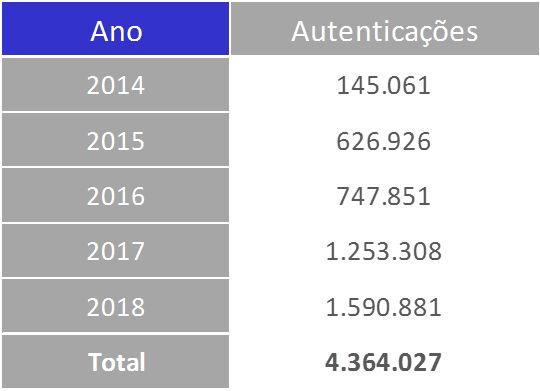
\includegraphics[width=0.5\textwidth]{img/authgov/authCC.png}
        \caption{Evolução do número de Autenticações realizadas através do Cartão de Cidadão.\cite{authGovStats}}
    \end{figure}
    
    \item \gls{cmd}
    
    Com a crescente adesão a serviços de autenticação baseadas em \emph{smartphones}, a utilização da Chave Móvel Digital tem vindo a ganhar tração cada vez maior nos últimos anos, provando ser uma alternativa complementar, bem como viável à utilização do Cartão de Cidadão como meio de autenticação primária.
    
    \begin{figure}[h]
        \centering
        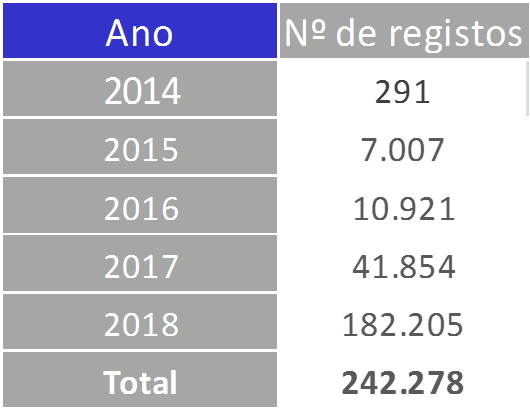
\includegraphics[width=0.45\textwidth]{img/authgov/authCMD.png}
        \caption{Evolução do número de Autenticações realizadas através da Chave Móvel Digital.\cite{authGovStats}}
    \end{figure}
\end{itemize}

\subsection{Funcionamento do Autenticação.Gov}

De acordo com o manual de Integração do \emph{Autenticação.Gov} providenciado pela \gls{ama}, existem 4 interações\cite{manualAuthGov} entre o \emph{Autenticação.Gov} e a entidade/serviço a aceder:

\begin{enumerate}
    \item O utilizador pretende aceder à área privada do portal de uma entidade, na qual é necessário que comprove a sua identidade;
    \item O portal da entidade delega a autenticação e redireciona o utilizador para o Auten-ticação.Gov, juntamente com um pedido de autenticação assinado digitalmente;
    \item O Autenticação.Gov valida o pedido de autenticação recebido e solicita a autenticação do utilizador com recurso ao seu Cartão de Cidadão pedindo a inserção do seu PIN de autenticação. Durante este processo, o Autenticação.Gov efetua as seguintes operações internas:
    \begin{itemize}
        \item Valida as credenciais do utilizador com recurso à PKI do Cartão de Cidadão via \gls{ocsp}.
        \item Obtém atributos que sejam solicitados pelo portal da entidade junto dos vários fornecedores de atributos qualificados. Esta operação é efetuada via Plataforma de Interoperabilidade. Este processo pode incluir a obtenção de dados da Fe-deração de Identidades ou de outras Entidades.
    \end{itemize}
    \item A identificação e atributos do utilizador são autenticadas e assinados digitalmente pelo Autenticação.Gov, após o que redireciona o utilizador de volta ao portal da entidade original. Cabe à entidade a validação das credenciais do Autenticação.Gov e utilização dos atributos do cidadão.
\end{enumerate}

\cleardoublepage
\subsubsection{SAML 2.0}

O \gls{saml} define um padrão standard para a troca de informação segura entre diversas entidades na Web.

Mais precisamente, o \gls{saml} define um framework \gls{xml} para a troca de asserções de informação entre entidades. 

\begin{displayquote}
"...to define, enhance, and maintain a standard XML-based framework for creating and
129 exchanging authentication and authorization information."
\\[5pt]
\rightline{{-- Security Assertion Markup Language V2.0 Technical Overview\cite{hughes2005security}}}
\end{displayquote}

A versão 2.0 do \gls{saml} foi aprovada pela \gls{oasis} em 2005, modificando o standard de tal forma, que implementações baseadas na versão prévia (versão 1.1) eram incompatíveis com o novo standard.

Na especificação técnica do \gls{saml} existem dois \emph{providers}:

\begin{itemize}
    \item \emph{Identity provider}: faculta a autenticação, verificando a identidade do utilizador, procedendo ao envio de informação para o \emph{Service provider}, juntamente com os níveis de acesso do utilizador.
    \item \emph{Service provider}: requesita a autenticação ao \emph{Identity provider} de modo a proceder à autorização do utilizador.
\end{itemize}

\begin{figure}[h]
    \centering
    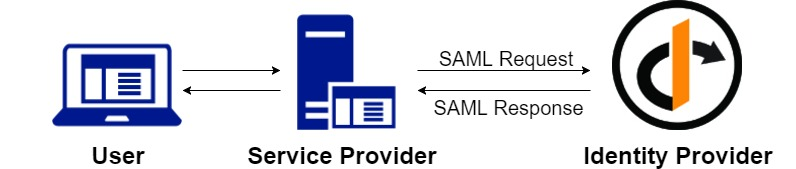
\includegraphics[width=\textwidth]{img/saml/samlproviders.jpg}
    \caption{Interação entre o utilizador e os respetivos \emph{Providers}. \cite{samlProviderPic}}
\end{figure}

Devido à especificação do \gls{saml}, este permite a utilização de \gls{sso}, ou seja, após um único login do utilizador, essas mesmas credenciais podem ser reutilizadas para proceder ao \emph{login} noutros \emph{Service Providers}.

De modo a realizar comunicação entre os \emph{providers} é utilizado um documento \gls{xml}, conhecido por \emph{SAML Assertion}. Existem 3 tipos de \emph{Assertions}:

\begin{enumerate}
    \item \emph{Authentication}: forcene identificação do utilizador em questão, providenciando dados como a hora a que o login foi realizado e que tipo de autenticação foi utilizada (por exemplo: Cartão de Cidadão).
    \item \emph{Attribution}: transmite atributos \gls{saml} (um atributo \gls{saml} trata-se de um formato de dados responsável pela transmição de informação sobre o utilizador) para o \emph{Service Provider}.
    \item \emph{Authorization}: reporta se o utilizador está autorizado a utilizar o serviço em questão, ou se este foi negado autorização pelo \emph{Identity Provider}.
\end{enumerate}

Em suma, o \gls{saml} funciona através do partilha de informação sobre utilizadores, login e atributos entre ambos os \emph{Providers}. 

Após ser realizado um login com o auxílio do \emph{Identity Provider}, este pode enviar atributos SAML para o \emph{Service Provider} quando o utilizador tenta aceder a certos serviços. Por ventura, o \emph{Service Provider} requesita autorização e autenticação ao \emph{Identity Provider}.


%\subsubsection{SSL/TLS}

\cleardoublepage
\section{Autenticação de pedidos via API}

No âmbito do projeto \gls{clav} é disponibilizada uma \gls{api} pública de modo a serem feitas \emph{queries} à base de dados.

De modo a estas chamadas, bem como controlar uso indevido da mesmas, foi necessário implementar autenticação e controlo através de \gls{jwt}\footnote{Mais informação em \url{https://jwt.io}}.

A essência do \gls{jwt} assenta no facto do token ser ou não válido, ou seja, se este já expirou ou foi revogado. A implementação deste token foi feita de forma a ser possível monitorizar quem está a fazer chamadas à \gls{api}, podendo a qualquer altura revogar autorização para tal, bem como a auto-revogação após 30 dias.

Estes cuidados ajudam a evitar problemas, tais como ataques à \gls{api} através de sucessivas chamadas num curto espaço de tempo, o que provoca uma sobrecarga no sistema.

\subsection{Introdução ao JSON Web Token}

\begin{figure}[h]
    \centering
    
\includegraphics[width=0.75\textwidth]{img/jwt/jwtlogo.png}
    \caption{Logótipo do \emph{JSON Web Token}. \cite{jwtLogo}}
\end{figure}

Mas o que define um \gls{jwt}? Um \gls{jwt} é nada mais que um \emph{standard RFC 7519}\cite{jones2015json}\cite{peyrott2016jwt}\footnote{Mais informação em \url{https://tools.ietf.org/html/rfc7519}} desenvolvido para a troca de pedidos em ambientes cujo espaço é limitado. 

Atualmente, este é utilizado nos frameworks web mais populares, devido ao seu tamanho compacto, simplicidade e usabilidade, tornando-o no perfeito candidato para diversas aplicações.

\cleardoublepage
\subsubsection{Funcionamento do JSON Web Token}

Um \emph{JSON Web token} é composto por 3 elementos distintos (quebras de linha inseridas para melhorar a leitura), separados por um ponto (\textbf{ . }) entre cada elemento:

\begin{center}
    \textbf{\textcolor{red}{eyJhbGciOiJIUzI1NiIsInR5cCI6IkpXVCJ9}.\\
    \textcolor{green}{eyJzdWIiOiIxMjM0NTY3ODkwIiwibmFtZSI6Ik\\9jdMOhdmlvIE1haWEiLCJudW1BbHVubyI6NzEzNjl9}.\\
    \textcolor{blue}{SneQiuAGUW9aTpxlNNbMkEoYNj7v4-Sw\_5jl134-hosk}}
\end{center}

Embora seja impossível retirar alguma informação útil do \emph{token} exemplificado anteriormente, este contem informação extremamente útil, tendo sido gerado através da seguinte informação:

\begin{itemize}
    \item Header (representado a vermelho).
    \begin{verbatim}
    {
      "alg": "HS256",
      "typ": "JWT"
    }
    \end{verbatim}
    
    Todos os \emph{JSON Web Token} possuem um header. Este elemento estabelece qual o algoritmo utilizado, se o \gls{jwt} foi assinado ou encriptado e por norma, como proceder ao parse do resto do \gls{jwt}.
    
    O único atributo obrigatório num \gls{jwt} é o \emph{alg}, sendo que em \gls{jwt} que não foram encriptados este valor é \textbf{none}, sendo que neste exemplo foi utilizada a encriptação \textbf{HS256}, ou seja, \gls{hmac} com o auxílio de \gls{sha256}.
    
    Existem tambem atributos opcionais, tais como \emph{typ}, cuja função é distinguir entre o \gls{jwt} e outros tipos de dados que possam ser transmitidos no mesmo formato\footnote{Tipos de dados transmissíveis: \url{http://www.iana.org/assignments/media-types/media-types.xhtml}}, sendo que neste exemplo é transmitido um \emph{JWT} e \emph{cty}, que apenas é utilizado quando existem aninhamento de \gls{jwt} dentro de outro(s) \gls{jwt}.
    
    Após o uso do algoritmo \textbf{HS256}, a informação acima representada é transcrita sobre a forma da seguinte string:
    
    \begin{center}
        \textbf{\emph{eyJhbGciOiJIUzI1NiIsInR5cCI6IkpXVCJ9}}
    \end{center}
    
    \newpage
    \item Payload (representado a verde).
    \begin{verbatim}
    {
      "sub": "1234567890",
      "name": "Octavio Maia",
      "numAluno": 71369
    }
    \end{verbatim}
    
    O payload é o elemento responsável pelo armazenamento de todo e qualquer dado do utilizador. Como o header, este elemento segue o formato \emph{JSON}, embora que todos os atributos presentes no payload sejam de natureza opcional, ao contrário do header que possui pelo menos um atributo de cariz obrigatório.
    
    De acordo com a especificação do payload, existem 7 atributos registados, sendo que neste exemplo apenas existe um, designado por \emph{sub}. Este atributo contem informação sobre quem se trata a informação contida neste \gls{jwt}, sendo que para tal efeito, este atributo é de cariz único na aplicação em questão.
    
    Os atributos designados por \emph{name} e \emph{numAluno} são designado por atributos não registados, podendo conter qualquer tipo de informação representável sobre a forma de string.
    
    No âmbito do projeto \gls{clav} são utilizados outros atributos registados, sendo o de maior importância o atributo \emph{exp}, cuja função é representar uma data específica, seguindo o formato \emph{"seconds since epoch"}\footnote{Definido pela \gls{posix} em \url{http://pubs.opengroup.org/onlinepubs/9699919799/basedefs/V1_chap04.html##tag_04_15}}, após a qual o \gls{jwt} é considerado inválido.
    
    A informação acima representada anteriormente é transcrita sobre a forma da seguinte string:
    
    \begin{center}
        \textbf{\emph{eyJzdWIiOiIxMjM0NTY3ODkwIiwibmFtZSI6Ik\\9jdMOhdmlvIE1haWEiLCJudW1BbHVubyI6NzEzNjl9}}
    \end{center}
    
    \newpage
    \item Assinatura (representado a azul).
    \begin{verbatim}
    HMACSHA256(
      base64UrlEncode(header) + "." +
      base64UrlEncode(payload),
      secretKey  
    )
    \end{verbatim}
    
    Embora a definição de \gls{jwt} apenas abranja os dois elementos previamente estudados, o terceiro elemento apenas tem como função a desencriptação do \gls{jwt} para efeitos de \emph{parsing}.
    
    Por norma é utilizado uma variante do algoritmo \emph{Base64}, designada por \emph{Base64-URL}. Para encriptar a assinatura, são concatenadas 3 strings que foram sujeitas ao codificação via \emph{Base64-URL}.
    
    \begin{verbatim}
        [Base64-URL header].[Base64-URL payload].[secretKey]
    \end{verbatim}
    
    O resultado desta concatenação e posterior encriptação via \textbf{HS256} é a seguinte string:
    
    \begin{center}
        \textbf{\emph{SneQiuAGUW9aTpxlNNbMkEoYNj7v4-Sw\_5jl134-hosk}}
    \end{center}
\end{itemize}

%\cleardoublepage
%\subsubsection{Vulnerabilidades do JSON Web Token}

\cleardoublepage
\subsection{Autenticação de pedidos à API}

De modo a proceder à autenticação de pedidos à \gls{api}, irá ser implementado um sistema baseado em \emph{JSON Web Tokens}.

Esta implementação seguirá as normas propostas pelo \emph{"OAuth 2.0 Authorization Framework: Bearer Token Usage"}\cite{rfc6750}, utilizando para o efeito um header HTTP do tipo \emph{Authorization}, com esquema de autenticação \emph{Bearer}\footnote{Mais informação em \url{https://www.iana.org/assignments/http-authschemes/http-authschemes.xhtml}}.

\begin{figure}[h]
    \centering
    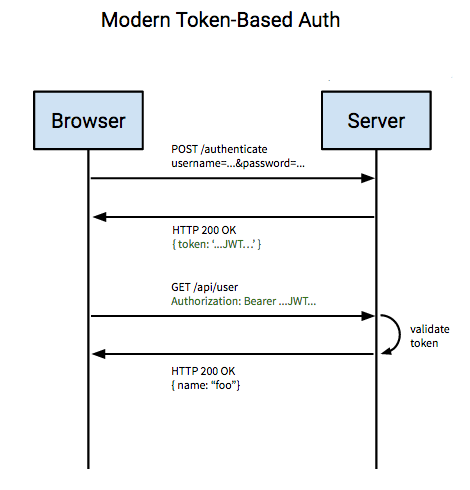
\includegraphics[width=0.75\textwidth]{img/jwt/diagramafluxoJWT.png}
    \caption{Diagrama correspondente à autenticação baseda em tokens. \cite{jwtDiagram}}
\end{figure}

O sistema de autenticação a ser implementado seguirá o diagrama previamente descrito, ou seja:

\begin{enumerate}
    \item É realizada a autenticação de um elemento externo no nosso servidor.
    \item Caso a autenticação tenha sucesso, irá ser devolvido um \gls{jwt} que irá servir de \emph{API Key} para a autenticação de chamadas à mesma.
    \item Cada vez que é feita uma chamada à \gls{api}, o token presente no campo \emph{Authorization} irá ser validado.
    \item Caso este seja validado com sucesso, irá ser retornado o output da chamada à API solicitada.
\end{enumerate}

Outra possibilidade de implementação é descrita a seguir, onde no servidor 3 (neste caso, o servidor responsável por correr o projeto \gls{clav}), possui uma lista de \emph{API Key} válidas (neste caso, \gls{jwt}).

\begin{figure}[h]
    \centering
    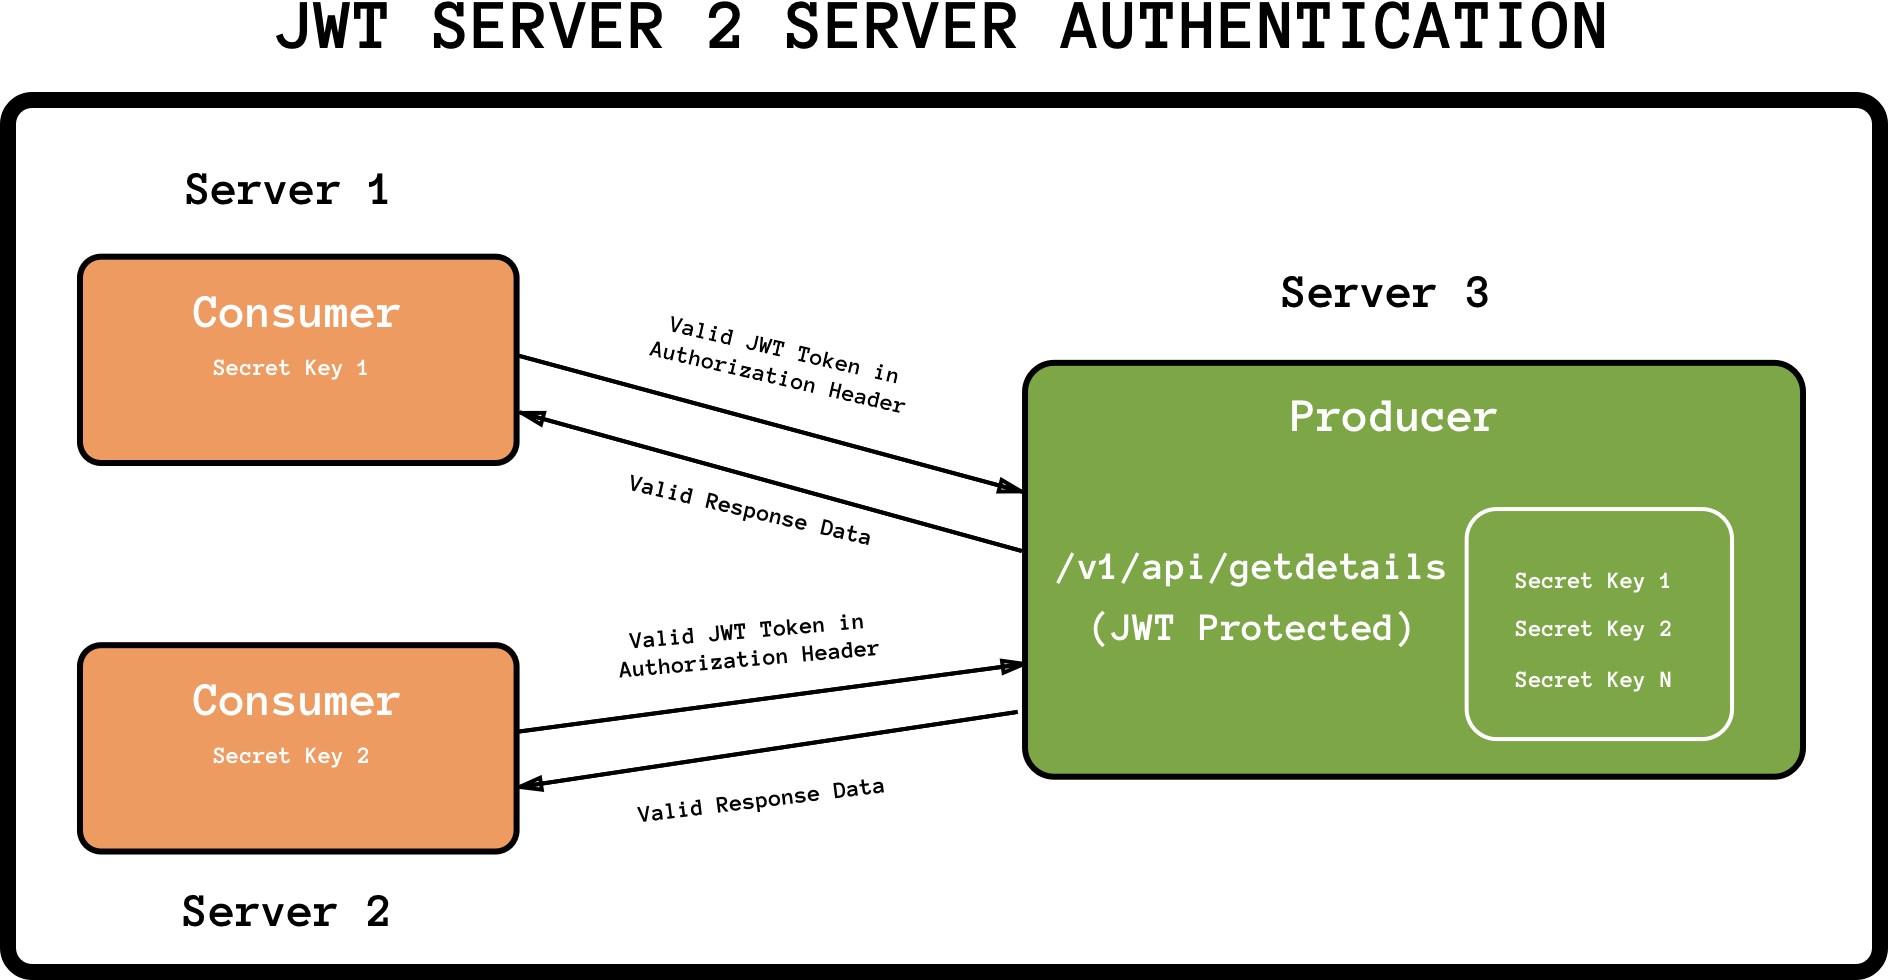
\includegraphics[width=\textwidth]{img/jwt/jwtAPI.png}
    \caption{Representação da utilização de \emph{JSON Web Token} para autenticação de pedidos à API. \cite{jwtAPI}}
\end{figure}

Cada vez que uma chamada à \gls{api} é feita, irá ser verificado se o \emph{token} dos utilizadores (representados por consumidores na imagem), está presente na lista de chaves pré validadas.

\cleardoublepage
\section{Autenticação backend}

Aqui falo das diversas funçoes de middleware que verificam se o utilizador tem nível de acesso adequado? Nao parece haver muito mais para dizer